
\subsection*{1.}

Si la tangente est horizontale, le nombre dérivé \(f'(1)\) est nul.

\subsection*{2.}

Cette tangente est la droite \((AC)\), donc son équation est \(-x + y = 2\) ou \(y = x + 2\).

\subsection*{3.}

\(f\) est un produit de fonctions dérivables sur \([-10\,;\,2]\), et sur cet intervalle :
\[
f'(x) = -\e^x + (2 - x) \e^x = \e^x (-1 + 2 - x) = \e^x(1 - x).
\]

\subsection*{4.}

\begin{center}
\begin{tikzpicture}
\tkzTabInit[lgt=3.5, espcl=4.5]{$x$ / 1, {$e^x$} / 1, {$1-x$} / 1, {Signe de $f'(x)$} / 1, {$f$} / 2}{${-10}$, ${1}$, ${2}$}
\tkzTabLine{,+,,+,}
\tkzTabLine{,+,0,-,}
\tkzTabLine{,+,0,-,}
\tkzTabVar{-/{$12\e^{-10} \approx 0{,}0005$},+/{$\e^1 \approx 2{,}728$},-/{$0$}}{/}
\end{tikzpicture}
\end{center}

\subsection*{5.}

Si \(\Delta\) est cette tangente, on sait qu'une équation de celle-ci est :
\[
M(x\,;\,y) \in \Delta \iff y - f(2) = f'(2)(x - 2).
\]
Avec \(f(2) = 0\) et \(f'(2) = -\e^2\), l'équation devient :
\[
M(x\,;\,y) \in \Delta \iff y = -\e^2(x - 2) \quad \text{ou} \quad y = \e^2(2 - x).
\]

